%	CHAP EdgeR
%----------------------------------------------------------------------------------------

\chapterimage{blue-chapter-head_4-reduced.pdf} % Chapter heading image

\chapter{EdgeR}\label{chap:EdgeR}
\section{Understanding Language Composition}

The EdgeR language (\texttt{org.campagnelab.metaR.edgeR}) has been developed as a illustration of language composition with MetaR. When you import the \texttt{org.campagnelab.metaR} devkit into MPS, you are able to create analyses and the statements described in the previous Chapter. If you tried to enter the \texttt{edgeR} alias, the error shown in Figure~\ref{fig:ErrorEdgeRNotDefined} would appear. The reason is that by default, MetaR does not provide an EdgeR statement. 
\begin{SCfigure}
  \centering
  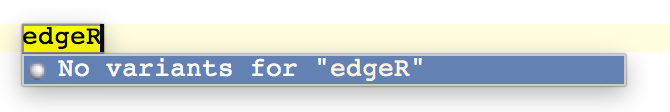
\includegraphics[width=\figWidthNarrow]{figures/edgeR_error-nosuchstatement.png}
\caption[Error When Typing the EdgeR Alias.]{\textbf{Error When Typing the EdgeR Alias.} The \texttt{EdgeR} statement is not yet defined.}
\label{fig:ErrorEdgeRNotDefined}
\end{SCfigure}

If you now also import the \texttt{org.campagnelab.metaR.edgeR} language (use \keys{\cmd+L} and import the \texttt{edgeR} language), you will be able to use the \texttt{edgeR} statement. A new EdgeR statement is shown in Figure~\ref{fig:NewEdgeRStatement}. Adding the EdgeR language to MetaR contributes a new kind of Analysis statement, which becomes available through auto-completion. From a user point of view, importing languages is all that is required to extend MetaR with new language constructs. This new statement can be configured by the user and will generate R code together with the other statements. This happens seamlessly and requires no other configuration than declaring that the model uses another language.


\begin{figure}[h!tbp]
  \centering
  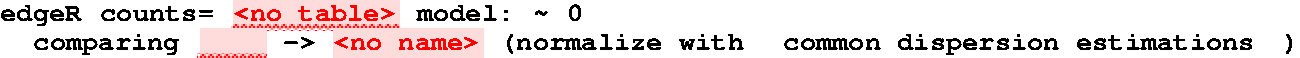
\includegraphics[width=\figWidthWide]{figures/NewEdgeRStatement.pdf}
\caption[New EdgeR Statement.]{\textbf{New EdgeR Statement.} A new EdgeR statement created after you have added the \texttt{org.campagnelab.metaR.edgeR} language to the model's MPS Used Languages.}
\label{fig:NewEdgeRStatement}
\end{figure}

\section{The edgeR Statement}
The edgeR statement performs tests of differential expression using read counts contained in a table of data. The statement has the following attributes.

\paragraph{counts table}
The table must contain columns annotated with the ``counts'' group. Bind this table reference to a table that contains non-normalized read counts.

\paragraph{model}
You can use the model attribute to enter a linear model. EdgeR will use this model to model the mean and variance of the data. You can enter a linear model by typing \texttt{+} followed by the name of a group usage attached to the counts table. Repeat to add multiple factors to the model. 
\begin{remark}
EdgeR will use an exact test when the model has one factor. but will use a Generalized Linear Model (GLM) when the model has more than one factor. This is handled transparently.
\end{remark}

\paragraph{comparing}
The comparing attribute makes it possible to define the statistics that should be tested for difference with zero. After you have defined a model with several factors (corresponding to group usage), the factor levels (corresponding to group names) will be offered for auto-completion. The factor level name stands for the average of the columns annotated with the group. See Figure~\ref{fig:EdgeRExample} for an example. 

\paragraph{normalize with}

EdgeR supports three types of normalization methods, which estimate variance/dispersion in different ways:

\begin{itemize}
  \item common dispersion 
  \item trended dispersion
  \item tagwise dispersion
\end{itemize}

Place the cursor on the keyword following normalize with and use auto-completion to switch from one type of normalization method to another. The the EdgeR Bioconductor documentation \url{http://www.bioconductor.org/packages/release/bioc/html/edgeR.html} for details about these approaches.

\section{Example}
Figure~\ref{fig:EdgeRExample} presents an example where the edgeR statement is configured with a model (one factor: \texttt{LPS}) to call differences between columns labeled with the groups \texttt{LPS=YES} and \texttt{LPS=NO}.

\begin{figure}[h!tbp]
  \centering
  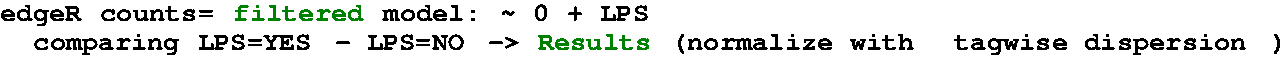
\includegraphics[width=\figWidthWide]{figures/EdgeRExample.pdf}
\caption[EdgeR Example.]{\textbf{EdgeR Example.}}
\label{fig:EdgeRExample}
\end{figure}
